\documentclass[oneside,a4paper,11pt]{book}
\usepackage[utf8]{inputenc}
\usepackage{svg}
\usepackage[italian]{babel}
\usepackage{float}
\usepackage{fancyvrb}
\usepackage{titling}
\usepackage[margin=1in,footskip=0.25in]{geometry}
\usepackage{listings}
\usepackage[DIV=12,BCOR=2mm,headinclude=true,footinclude=false]{typearea}
\usepackage{color, colortbl,xcolor}
\usepackage[hidelinks]{hyperref}
\usepackage{tcolorbox}
\usepackage{chngcntr}
\usepackage{diagbox}
\usepackage{calc}
\usepackage{amssymb}
\usepackage{subcaption}
\usepackage{amsthm}
\usepackage{amsfonts}
\usepackage{mathtools}
\usepackage{parskip}
\usepackage{cancel}
\usepackage{forest}
\usepackage{listings}
\usepackage{mathrsfs}
\usepackage{enumitem}
\usepackage{makecell}
\usepackage{tikz}
\usepackage{pgfplots}
\pgfplotsset{compat=1.18}
\usepackage{fancyhdr}
\fancypagestyle{plain}{\fancyhf{}\renewcommand{\headrulewidth}{0pt}}
\pagestyle{fancy}
\fancyhf{}% Clear header/footer
\fancyhead[L]{\nouppercase\leftmark}
\fancyhead[R]{\thepage}
\usetikzlibrary{positioning,shapes.geometric,arrows.meta,matrix,automata,decorations.pathmorphing,patterns,decorations.pathreplacing,shapes.multipart,calc,snakes}
\usetikzlibrary{arrows.meta, backgrounds, chains, positioning, shapes.geometric, shapes.multipart}
\tcbuselibrary{skins}
\counterwithin{figure}{section}
%Nuovi comandi
\newcommand\myeq{\stackrel{\mathclap{\normalfont\mbox{def}}}{=}}
\newcommand\prodG{\stackrel{\mathclap{\normalfont\mbox{\tiny{G}}}}{\Longrightarrow}}
%asmthm
\newlength{\marginlabelsep}\setlength{\marginlabelsep}{0.5em}
\newtheoremstyle{italicstyle} %% Name
  {} %% <- Space above (empty = default = \topsep = 8.0pt plus 2.0pt minus 4.0pt)
  {} %% <- Space below (empty = default = \topsep = 8.0pt plus 2.0pt minus 4.0pt)
  {\itshape} %% <- Body font
  {} %% <- Indent amount (empty = no indent, \parindent = just that)
  {\bfseries} %% <- Thm head font
  {} %% <- Punctuation after thm head
  {1pt} %% <- Space after thm head (or " " or \newline) (default: 5pt plus 1pt minus 1pt)
  {\vtop to 0pt{\llap{\thmname{#1}\hskip\marginlabelsep}
                \llap{\thmnumber{#2}\hskip\marginlabelsep}}\thmnote{#3\\}%
  }
\newtheoremstyle{normStyle} %% Name
  {} %% <- Space above (empty = default = \topsep = 8.0pt plus 2.0pt minus 4.0pt)
  {} %% <- Space below (empty = default = \topsep = 8.0pt plus 2.0pt minus 4.0pt)
  {\normalfont} %% <- Body font
  {} %% <- Indent amount (empty = no indent, \parindent = just that)
  {\bfseries} %% <- Thm head font
  {} %% <- Punctuation after thm head
  {1pt} %% <- Space after thm head (or " " or \newline) (default: 5pt plus 1pt minus 1pt)
  {\vtop to 0pt{\llap{\thmname{#1}\hskip\marginlabelsep}
                \llap{\thmnumber{#2}\hskip\marginlabelsep}}\thmnote{#3\\}%
  }
\theoremstyle{italicstyle}
\newtheorem{corollary}{Corollario}[section]
\newtheorem{notazione}{Notazione}[section]
\newtheorem{lemma}{Lemma}[section]
\newtheorem{definizione}{Definizione}[section]
\newtheorem{nota}{Nota}[section]
\newtheorem{exercise}{Esercizio}[section]
\theoremstyle{normStyle}
\newtheorem{exmp}{Esempio}[section]
\newtheorem{theorem}{Teorema}[section]
\newtheorem{proposizione}{Proposizione}[section]
\tcbuselibrary{listings,skins}
\newtcblisting{mylisting}[2][]{
    arc=0pt, outer arc=0pt,
    listing only, 
    title=#2,
    #1,
    listing options= {escapechar=|}
}

\newcommand{\myboxedtext}[2][rectangle,draw]{%
    \tikz[baseline=-0.6ex] \node [#1]{#2};}%
%%======================================================================
\title{Crittografia}
\author{\textit{Alessio Gjergji}}
\date{}
\begin{document}
\maketitle
\tableofcontents
\chapter{Tecniche crittografiche classiche}
\section{La differenza tra crittografia e steganografia}
La crittografia e la steganografia sono due tecniche per proteggere la
confidenzialità dei dati. 
La crittografia si basa sulla trasformazione
dei dati in modo che non siano leggibili, mentre la steganografia si
basa sulla segretezza dell'esistenza dei dati.

La crittografia ha come obiettivo quello di rendere illeggibili i dati,
non nasconde l'esistenza dei dati. La steganografia invece nasconde
l'esistenza dei dati, ma non li rende illeggibili.

Il problema della steganografia è che se si scopre l'esistenza dei dati,
si può facilmente decifrare il messaggio, compromettendo quindi l'intera 
comunicazione. La crittografia invece sfrutta algoritmi matematici conosciuti
per rendere illeggibili i dati, quindi anche se si conosce l'algoritmo di
codifica, non è possibile decifrare il messaggio senza la chiave.
\begin{tcolorbox}
    L'obiettivo è costruire un algoritmo crittografico dove la sicurezza 
    dipenda solo dalla segretezza della chiave e non dall'algoritmo sottostante.
\end{tcolorbox}
Possiamo dire quindi che un sistema è sicuro nel momento in cui il costo 
economico per decifrarlo è maggiore del valore dell'informazione che contiene.
\section{Cifrario di cesare}
Il cifrario di Cesare è noto come il primo e più semplice esempio di
cifrario a sostituzione. Fu utilizzato da Giulio Cesare e coinvolge la
sostituzione di ogni lettera dell'alfabeto con la lettera situata tre
posizioni più in basso nell'alfabeto. Ad esempio:

\begin{center}
\begin{tabular}{|c|c|}
\hline
\textbf{Plain} & \textbf{Ciphertext} \\
\hline
a & d \\
b & e \\
c & f \\
d & g \\
e & h \\
f & i \\
g & j \\
h & k \\
i & l \\
j & m \\
k & n \\
l & o \\
m & p \\
\hline
\end{tabular}
\hspace{2cm}
\begin{tabular}{|c|c|}
\hline
\textbf{Plain} & \textbf{Ciphertext} \\
\hline
n & q \\
o & r \\
p & s \\
q & t \\
r & u \\
s & v \\
t & w \\
u & x \\
v & y \\
w & z \\
x & a \\
y & b \\
z & c \\
\hline
\end{tabular}
\end{center}

È importante notare che l'alfabeto è avvolto in modo che la lettera
successiva a Z sia A. Ogni lettera dell'alfabeto viene quindi sostituita
dalla lettera che si trova a tre posizioni più in basso.

Il cifrario di Cesare è un esempio semplice ma storico di crittografia a
sostituzione. Può essere utilizzato per crittografare un messaggio
spostando ogni lettera di tre posizioni nell'alfabeto.

L'algoritmo utilizzato è il seguente:
\[
C = E(3, p) = (p + 3)\mod 26  
\]
Lo shift potrebbe essere un valore generico $k$, quindi l'agoritmo generalizzato 
è:
\[
C = D(k, p) = (p + k)\mod 26  
\]
ove $k$ prende un valore nel compreso tra $1$ e $25$. L'algoritmo di 
decifrazione è simile:
\[
  p = D(k, C) = (C - k)\mod 26  
\]

Il problema di questo algorithm è che ci sono solo $26$ chiavi possibili,
quindi è molto semplice decifrarlo con un attacco a \textbf{forza bruta}.
L'attacco avviene provando tutte le $26$ chiavi possibili e verificando
se il testo decifrato ha senso un senso. Se il testo decifrato non ha senso,
si prova con la chiave successiva. Se il testo decifrato ha senso, si è trovata
la chiave.

Questa tipologia di attacco sfrutta solamente la conoscenza del testo cifrato
e non del testo in chiaro, e questa tipologia di attacco è detta \textbf{known 
ciphertext attack}.

Se la decodifica viene fatta da noi essere umani, è possibile verificare che la 
codifica abbia senso conoscendo il significato del testo in chiaro, ovvero 
conoscendo la lingua in cui è scritto il testo. Se invece la decodifica viene
fatta da un computer, è necessario utilizzare un altro metodo per verificare
che il testo decifrato abbia senso.
Un computer per verificare che un testo abbia senso, può utilizzare un
\textbf{dizionario} e verificare che le parole del testo decifrato siano
presenti nel dizionario, o eseguire un analisi statistica delle parole del
testo decifrato attraverso l'analisi delle frequenze della lingua in questione.

\section{Cifrario  monoalfabetico}
Per rendere più difficile l'attacco a forza bruta, bisogna ragionare sul fatto che 
l'obiettivo è quello di rendere la combinazioni di chiavi possibili molto grande.

Con solo $25$ chiavi possibili, il cifrario di Cesare è molto lontano
dall'essere sicuro. Un aumento drammatico dello spazio delle chiavi
può essere ottenuto consentendo una sostituzione arbitraria. Prima
di procedere, definiamo il termine \textbf{permutazione}.
\begin{tcolorbox}[title = {Permutazione}]
Una permutazione di un insieme finito di elementi $S$ è una
sequenza ordinata di tutti gli elementi di $S$, con ciascun elemento
che appare esattamente una volta. Ad esempio, se $S = \{a, b, c\}$, ci
sono sei permutazioni di $S$:
\end{tcolorbox}
\[
abc, acb, bac, bca, cab, cba
\]
In generale, ci sono $n!$ permutazioni di un insieme
di $n$ elementi, poiché il primo elemento può essere scelto in uno
dei modi $n$ possibili, il secondo in $n - 1$ modi, il terzo
in $n - 2$ modi e così via.

\begin{center}
\begin{tabular}{|c|c|}
\hline
\textbf{Plain} & \textbf{Ciphertext} \\
\hline
    a & p \\
    b & o \\
    c & l \\
    d & k \\
    e & r \\
    f & s \\
    g & t \\
    h & a \\
    i & h \\
    j & b \\
    k & d \\
    l & c \\
    m & v \\
\hline
\end{tabular}
\hspace{2cm}
\begin{tabular}{|c|c|}
\hline
\textbf{Plain} & \textbf{Ciphertext} \\
\hline
    n & g \\
    o & e \\
    p & f \\
    q & z \\
    r & x \\
    s & w \\
    t & y \\
    u & i \\
    v & m \\
    w & n \\
    x & q \\
    y & j \\
    z & u \\
    \hline
\end{tabular}
\end{center}

Se invece la linea ciphertext può essere qualsiasi permutazione
dei $26$ caratteri alfabetici, allora ci sono $26!$ o più di $4 \times 10^{26}$
possibili chiavi. Questo è $10$ ordini di grandezza superiore allo
spazio delle chiavi per \verb|DES| e sembrerebbe eliminare le tecniche di
crittoanalisi a forza bruta. Un approccio del genere è chiamato
cifrario di sostituzione monoalfabetica, perché viene utilizzato
un singolo alfabeto cifrato (\textit{mappatura dall'alfabeto in chiaro
all'alfabeto cifrato}) per ogni messaggio.

Purtroppo, questo schema è ancora vulnerabile ad altri tipi di attacchi,
come per esempio l'\textbf{analisi delle frequenze}.
Come primo passo, può essere determinata la frequenza relativa delle
lettere e confrontata con una distribuzione di frequenza standard per
la lingua in questione.
Se il messaggio fosse abbastanza lungo, questa tecnica da sola potrebbe
essere sufficiente, ma in caso di messaggi più corti,
non possiamo aspettarci una corrispondenza esatta.

Ci sono diverse modalità per procedere in questo punto. Potremmo fare alcune assegnazioni
provvisorie e iniziare a completare il testo in chiaro per vedere se assomiglia a uno scheletro
ragionevole di un messaggio.

Un approccio più sistematico è cercare altre regolarità. Ad esempio,
potrebbero essere noti alcuni termini nel testo. Oppure potremmo cercare sequenze ripetute di lettere
cifrate e cercare di dedurne le corrispondenti lettere in chiaro.

Un potente strumento è rappresentato dalla frequenza delle combinazioni di due lettere, 
chiamate \textbf{bigrammi}. Per esempio, in inglese, le lettere \verb|th| sono molto più
comuni di \verb|tx|, quindi se vediamo una combinazione di lettere che è molto più comune
di altre, possiamo dedurre che probabilmente corrisponde a \verb|th|.

Concludiamo che i cifrari monoalfabetici sono facili da decifrare perché riflettono i dati di frequenza
dell'alfabeto originale.
\section{Cifrario di Playfair}
Il cifrario di crittografia a più lettere più conosciuto è il cifrario di
\textit{Playfair}, che tratta i digrammi nel testo in chiaro come unità singole e li traduce
in digrammi nel testo cifrato. L'algoritmo di \textit{Playfair} si basa sull'uso di una matrice
$5 \times 5$ di lettere costruita utilizzando una parola chiave. Ecco un esempio, risolto da Lord Peter Wimsey nel
romanzo ``Have His Carcase" di \textit{Dorothy Sayers}:

\begin{center}
    \begin{tikzpicture}[font=\ttfamily\small]
        \matrix (playfair) [matrix of nodes,nodes={draw,minimum size=12mm,anchor=center},column sep=-\pgflinewidth,row sep=-\pgflinewidth]{
            |[fill=gray!20]| M & |[fill=gray!20]| O & |[fill=gray!20]| N & |[fill=gray!20]| A & |[fill=gray!20]| R \\
            |[fill=gray!20]| H & |[fill=gray!20]| Y & B & C & D \\
            E & F & G & I & K \\
            L & P & Q & S & T \\
            U & V & W & X & Z \\
        };
      \end{tikzpicture}
    \end{center}
In questo caso, la parola chiave è \textit{monarchia}. La matrice viene costruita riempiendo
le lettere della parola chiave (\textit{senza duplicati}) da sinistra a destra e dall'alto verso
il basso, e poi riempiendo il resto della matrice con le lettere rimanenti in ordine alfabetico.
Le lettere \verb|I| e \verb|J| contano come una sola lettera. Il testo in chiaro viene crittografato
due lettere alla volta, secondo le seguenti regole:
\begin{enumerate}
    \item Le lettere ripetute nel testo in chiaro che si trovano nella stessa coppia 
    vengono separate da una lettera di riempimento, come ad esempio \textit{x}, quindi \textit{balloon} 
    verrebbe trattato come \texttt{BA LX LO ON}.
    \item Due lettere nel testo in chiaro che si trovano nella stessa riga della matrice
    vengono ciascuna sostituite dalla lettera a destra, con il primo elemento della riga
    che segue ciclicamente l'ultimo. Ad esempio, \texttt{AR} viene crittografato come \texttt{RM}.
    \item Due lettere nel testo in chiaro che si trovano nella stessa colonna vengono ciascuna
    sostituite dalla lettera sottostante, con l'elemento superiore della colonna che segue
    ciclicamente l'ultimo. Ad esempio, \texttt{MU} viene crittografato come \texttt{CM}.
    \item In caso contrario, ogni lettera nel testo in chiaro nella coppia viene sostituita
    dalla lettera che si trova nella stessa riga e nella colonna occupata dall'altra lettera
    nel testo in chiaro. Quindi, \texttt{HS} diventa \texttt{BP} e
    \texttt{EA} diventa \texttt{IM} (\textit{o \texttt{JM}}).
\end{enumerate}
Il cifrario Playfair rappresenta un grande passo avanti rispetto ai semplici cifrari monoalfabetici.
Per una cosa, mentre ci sono solo $26$ lettere, ci sono $26 \cdot 26 = 676$ digrammi, rendendo
più difficile l'identificazione dei digrammi individuali. Inoltre, le frequenze relative delle singole
lettere mostrano una gamma molto più ampia rispetto a quella dei digrammi, rendendo l'analisi delle
frequenze molto più difficile. Per queste ragioni, il cifrario Playfair è stato a lungo considerato
indistruttibile. È stato utilizzato come sistema standard sul campo dall'Esercito Britannico durante
la Prima Guerra Mondiale e ha ancora goduto di un notevole utilizzo da parte dell'Esercito degli Stati
Uniti e altre forze alleate durante la Seconda Guerra Mondiale.
Nonostante questo livello di fiducia nella sua sicurezza, il cifrario Playfair è relativamente facile
da decifrare, perché lascia la maggior parte delle caratteristiche statistiche del testo in chiaro
intatte. 
\section{Cifrario di Vigenère}
Il cifrario di \textit{Vigenère} è un cifrario a sostituzione polialfabetica che utilizza una serie
di cifrari monoalfabetici differenti basati su lettere di una parola chiave. Per esempio, se il testo 
che vogliamo cifrare è \textit{provadiv}, e la parola chiave è \textit{paswd}, allora il testo
cifrato sarà l'applicazione di quattro cifrari monoalfabetici differenti, come mostrato nella seguente
tabella:
\begin{center}
    \begin{tabular}{|c|c|c|c|c|c|c|c|c|}
    \hline
     \textbf{Testo in chiaro} & p & r & o & v & a & d & i & v \\
     \hline
     \textbf{Parola chiave} & p & a & s & w & d & p & a & s \\
     \hline
     \textbf{Testo cifrato} & e & r & g & r & s & i & u & k \\
     
     \hline
    \end{tabular}
\end{center}
In questo crittosistema l'analisi delle frequenze non è più efficace, in quanto le lettere
del testo cifrato non sono più distribuite secondo la distribuzione delle lettere del testo in chiaro.
Andando però a vedere le lettere ad una distanza pari alla lunghezza della parola chiave, si può
notare che le lettere sono distribuite secondo la distribuzione delle lettere del testo in chiaro.

Il problema è che la lunghezza della parola chiave è sconosciuta, ma è possibile risolvere questo
tentando di individuare la lunghezza della parola chiave. Una volta che la lunghezza della parola
chiave è stata individuata, è possibile risolvere il cifrario di Vigenère come se fosse un cifrario
monoalfabetico.
\section{Cifraro di Vernam}
Il cifrario di \textit{Vernam} è un cifrario a blocchi che utilizza una chiave casuale della stessa
lunghezza del messaggio da cifrare. La chiave casuale è combinata con il messaggio da cifrare
utilizzando l'operazione di \texttt{XOR} (\textit{\texttt{OR} esclusivo}). L'operazione di \texttt{XOR}
è una funzione logica
binaria che restituisce 1 se e solo se i due bit di input sono diversi. L'operazione di \texttt{XOR} è
associativa, commutativa e invertibile. Questo significa che se $a$, $b$ e $c$ sono bit, allora
$(a \oplus b) \oplus c = a \oplus (b \oplus c)$, $a \oplus b = b \oplus a$ e $a \oplus a = 0$.

Per esempio, se il messaggio da cifrare è \texttt{10101010} e la chiave casuale è \texttt{11001100},
allora il testo cifrato sarà \texttt{01100110}. Per decifrare il messaggio, è sufficiente applicare
l'operazione di \texttt{XOR} tra il testo cifrato e la chiave casuale. Per esempio, se il testo cifrato
è \texttt{01100110} e la chiave casuale è \texttt{11001100}, allora il testo in chiaro sarà
\texttt{10101010}.

Si tratta quindi di un cifrario crittografico basato sul cifrario di Vigenère, in cui la chiave di 
cifratura è lunga tanto quanto il testo in chiaro e viene utilizzata una sola volta, chiamato 
\textit{one-time pad}. 
\subsection{Proprietà di One-Time Pad}
Il cifrario di Vernam è un sistema crittografico perfetto, nel senso che il messaggio può essere
decifrato solamente conoscendo la chiave di codifica. \textit{One-Time Pad} ha le seguenti proprietà:
\begin{itemize}
    \item \textbf{Chiave Casuale}: La chiave utilizzata nel cifrario monouso è una sequenza 
    casuale di bit o caratteri, lunga quanto il messaggio da crittografare. Essendo completamente casuale, 
    non contiene alcuna struttura o pattern riconoscibile.
    
    \item \textbf{Lunghezza della Chiave}: La chiave deve essere della stessa lunghezza del messaggio 
    in chiaro. Questo significa che ogni messaggio richiede una chiave diversa e della stessa lunghezza.
    
    \item \textbf{Unicità}: Ogni chiave è utilizzata una sola volta. Dopo essere stata usata per crittografare
    o decifrare un messaggio, la chiave viene scartata e non viene mai riutilizzata.
    
    \item \textbf{Sicurezza Statistica}: La sicurezza del cifrario monouso deriva dalla sua totale casualità.
    Poiché la chiave è una sequenza casuale e unica per ogni messaggio, non esiste alcuna relazione statistica
    tra il testo cifrato e il testo in chiaro. Questo significa che il testo cifrato non fornisce alcuna
    informazione utile per violare il cifrario, rendendolo teoricamente indistruttibile.
\end{itemize}
Il cifrario monouso, noto come \textit{one-time pad} è considerato perfetto dal punto di vista statistico
e crittografico per due ragioni principali:

\begin{enumerate}
    \item \textbf{Casualità della Chiave:} La chiave nel cifrario monouso è una sequenza casuale di bit o caratteri.
    La casualità è fondamentale dal punto di vista statistico. In termini di probabilità, ogni bit o carattere nella
    chiave ha una probabilità del 50\% di essere $0$ o $1$ (\textit{in caso di bit}) o di essere una qualsiasi
    lettera nell'alfabeto (\textit{in caso di caratteri}). Questo fatto è rappresentato dalla distribuzione di
    probabilità uniforme.
   
    Formula della distribuzione uniforme per bit:
    \[ P(X = 0) = P(X = 1) = \frac{1}{2} \]

    Formula della distribuzione uniforme per caratteri:
    \[ P(X = x_i) = \frac{1}{n} \text{ per ogni } x_i \text{ nell'alfabeto di lunghezza } n \]

    Ad esempio, in un alfabeto di $26$ lettere, la probabilità di ciascuna lettera è $1/26$.

    Nel caso di una chiave di lunghezza $n$, la probabilità di una particolare sequenza di $n$ bit o caratteri
    è $1/2^n$ o $1/n^n$ rispettivamente. Poiché non vi è alcuna relazione nei bit o caratteri della chiave.

    \item \textbf{Unicità della Chiave:} Ogni chiave viene utilizzata una sola volta per crittografare
    o decrittografare un messaggio specifico e viene scartata dopo l'uso. Questo significa che non c'è alcuna
    relazione statistica tra il testo cifrato e il testo in chiaro. L'assenza di qualsiasi pattern o relazione
    è fondamentale dal punto di vista della teoria della probabilità.
\end{enumerate}
\section{Concatenazione di crittosistemi}
Una permutazione è un mapping iniettivo e suriettivo di un insieme in se stesso.
Una permutazione è una sostituzione che mappa ogni lettera dell'alfabeto in un'altra lettera.
Quindi:
\[
    \pi : \mathcal{A} \rightarrow \mathcal{A}
\]
sappiamo che è vulnerabile all'analisi delle frequenze, quindi possiamo applicare 
un sistema di concatenazione:
\[
  \pi_1 \circ \pi_2 \circ \pi_3 \circ \pi_4 \circ \pi_5  
\]
il problema è che la composizione di permutazioni è ancora una permutazione,
quindi è la stessa cosa chè l'eseguire un'unica permutazione $\pi$.
Varia quindi solo la rappresentazione della permutazione.
Per risolvere il problema serve un elemento aggiuntivo che non sia una permutazione,
ad esempio una trasposizione.
\section{Macchina a Rotori}
Una macchina a rotori è una macchina crittografica che sfrutta
la crittografia a sostituzione \textbf{polialfabetica}. La macchina è composta
da cilindri rotanti, ognuno con $26$ pin di input e $26$ pin di output,
ciascuno con connessioni interne che collegano input e output in modo
univoco. Un singolo cilindro crea una sostituzione monoalfabetica,
ruotando dopo ogni input, il che crea una sostituzione polialfabetica
con un periodo di $26$ caratteri.

La vera forza delle macchine a rotori emerge quando vengono utilizzati
più cilindri collegati in serie. Quando si preme un tasto, il cilindro
più vicino all'input ruota di una posizione, influenzando il successivo
e così via. Questa configurazione crea una vasta varietà di sostituzioni
alfabetiche, con un'enorme quantità di possibilità quando si utilizzano
più cilindri.

Questo schema crittografico rappresenta una sfida significativa per i
crittoanalisti poiché richiede un'enorme quantità di dati cifrati per
essere decifrato in modo significativo, rendendo molto difficile
l'analisi crittografica basata sulla frequenza delle lettere.

Tale sistema protegge dall'analisi delle frequenze poiché per $26^3$ permutazioni 
non è possibile fare un'analisi delle frequenze.
\begin{figure}[H]
    \centering
    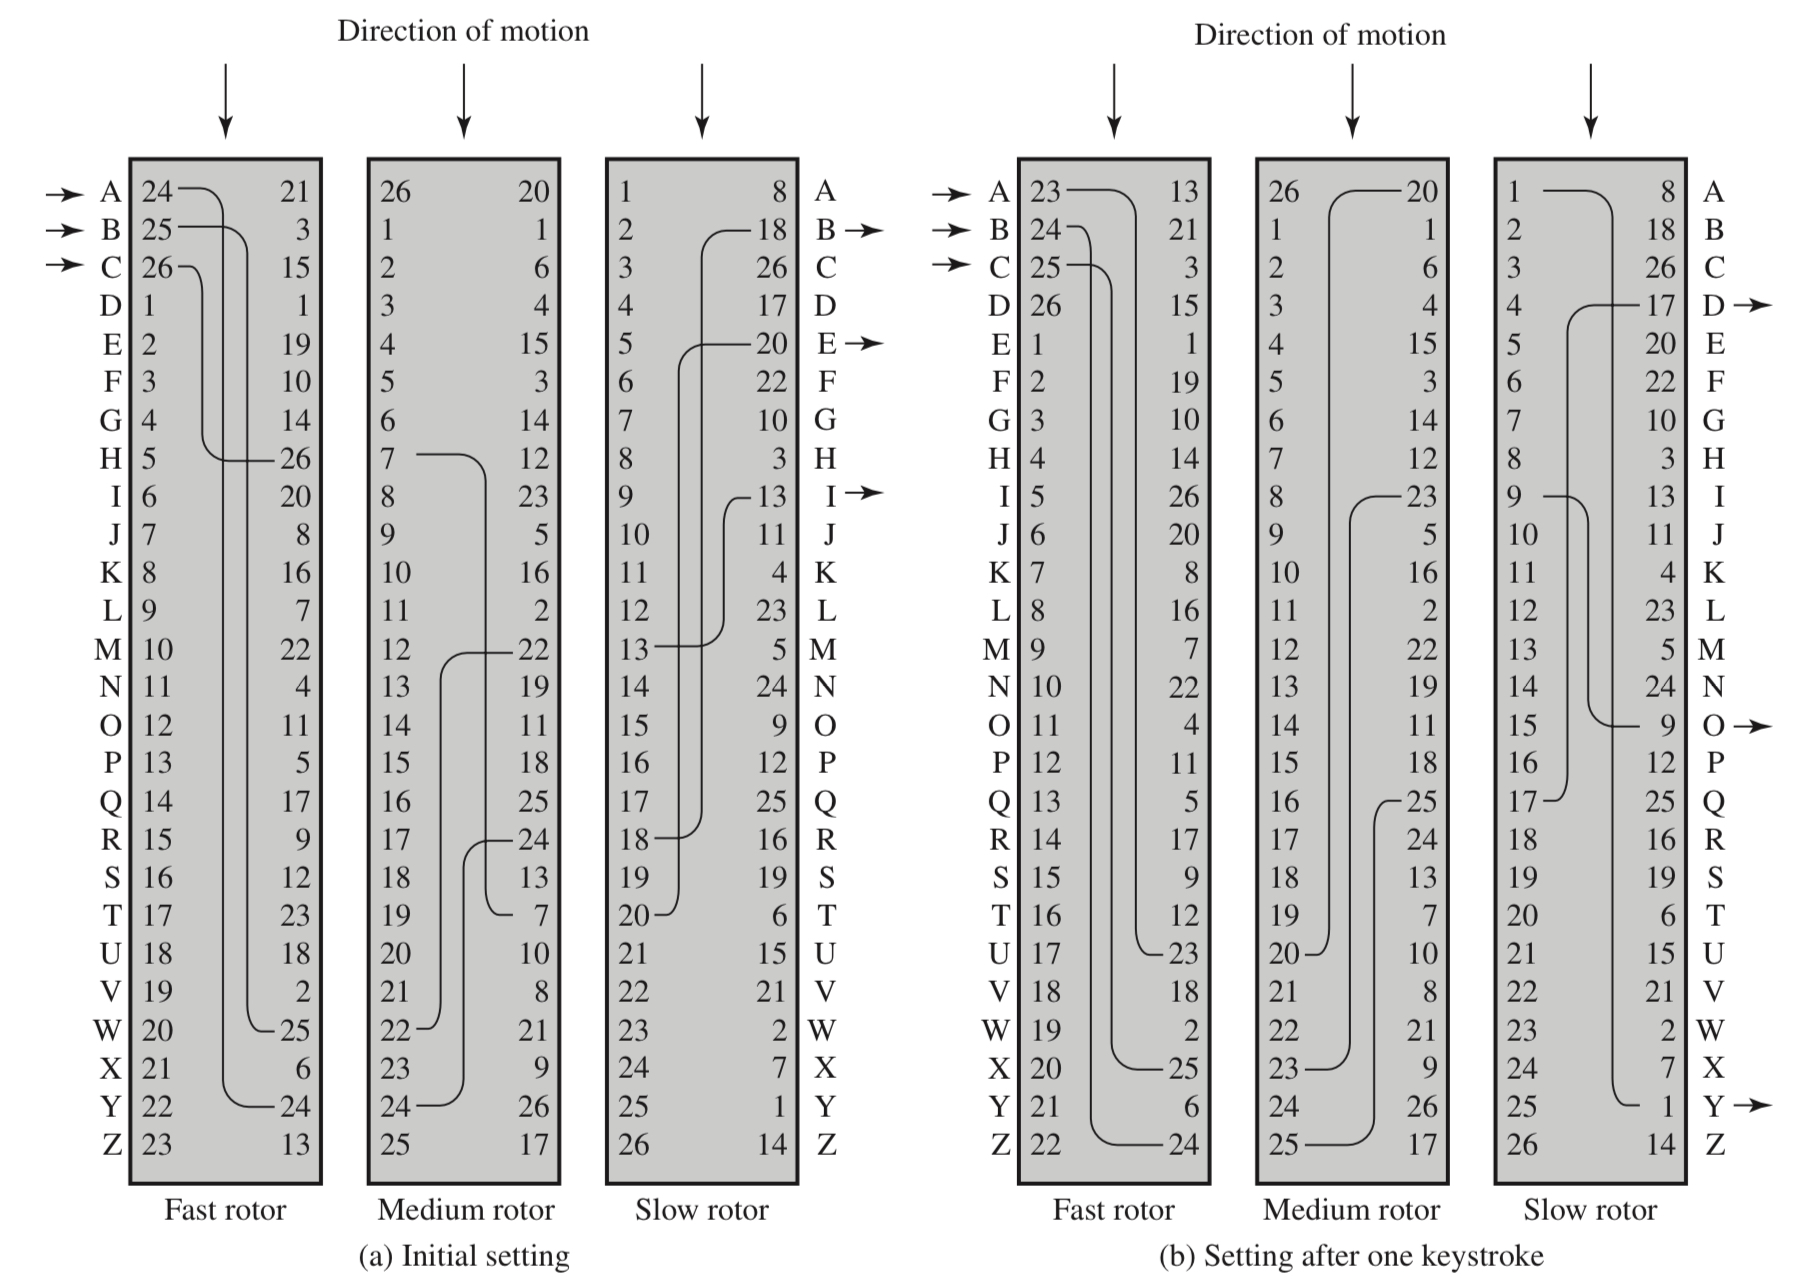
\includegraphics[width=0.8\textwidth]{img/Concatenazione_crittosistemi.png}
    \caption{Macchina a rotori}
\end{figure}

\subsubsection{Enigma}
La macchina Enigma è una macchina elettromeccanica portatile utilizzata per cifrare e decifrare
messaggi segreti. È stata utilizzata in Germania durante la seconda guerra mondiale.
La decodifica dei messaggi è molto complessa, vista la grande quantità di combinazioni possibili.

Se ho a una macchina che per essere decifrata ha bisogno di un tempo più alto della validità 
dei dati, allora posso dire che è sicura.

Il modo per decodificare i messaggi è stato fondamentale sapere che il messaggio iniziava con
una parola chiave, che era sempre la stessa. Sapendo questo, si poteva decodificare il messaggio
riducendo notevolmente l'insieme delle chiavi disponibili per la decodifica.
Conoscevano quindi il \textbf{plaintext}.

La concatenzione di crittosistemi è molto sicura, ma non è sicura contro gli attacchi
dove si conosce il plaintext.

\section{Classificazione dei livelli di sicurezza}
La classificazione si basa sulla difficoltà di violare il sistema, quindi sul tipo di 
attacchi a cui resiste.
\begin{itemize}
    \item \textbf{Known Cipher Text Attack}: l'attaccante conosce il testo cifrato.
    \item \textbf{Known Plaintext Attack}: l'attaccante vede il testo in chiaro e il corrispondente testo cifrato.
    \item \textbf{Chosen Plaintext Attack}: l'attaccante sceglie il testo in chiaro e conosce il corrispondente testo cifrato.
    \item \textbf{Adaptive Chosen Ciphertext Attack}: l'attaccante può continuamente scegliere il testo in chiaro e vedere il corrispondente testo cifrato.
\end{itemize}
La classifica è in base alla potenza che gli do nell'attaccarmi.
L'obiettivo è costruire un sistema che sia sicuro contro 
gli attacchi Adaptive Chosen Ciphertext Attack.
\section{Cifrari a flusso e a blocchi}
Un \textbf{cifrario a flusso} crittografa un flusso di dati digitali un bit
o un byte alla volta. Esempi di cifrari a flusso classici sono il
cifrario di Vigenère con autochiave e il cifrario di Vernam. Nell'ideale,
si utilizzerebbe una versione del cifrario di Vernam con one-time pad, in
cui lo stream di chiavi ha la stessa lunghezza dello stream di bit in chiaro.
Tuttavia, perché questo sia praticamente realizzabile, lo stream di chiavi deve
essere fornito in anticipo ad entrambi gli utenti attraverso un canale indipendente
e sicuro, il che può rappresentare una sfida logistica se il traffico dati
previsto è di grandi dimensioni.

Di conseguenza, per ragioni pratiche, il generatore di stream di bit deve
essere implementato come una procedura algoritmica, in modo che lo stream di
bit crittografico possa essere prodotto da entrambi gli utenti. In questo
approccio, il generatore di stream di bit è un algoritmo controllato dalla chiave
e deve produrre uno stream di bit crittograficamente robusto. I due utenti devono
condividere solo la chiave di generazione, e ognuno può generare lo stream di chiavi.

Un \textbf{cifrario a blocchi} tratta un blocco di testo in chiaro come un'entità
unica e produce un blocco di testo cifrato della stessa lunghezza. Di solito,
si utilizza una dimensione di blocco di $64$ o $128$ bit. Allo stesso modo del 
cifrario a flusso, i due utenti condividono una chiave di crittografia simmetrica.
Utilizzando alcune delle modalità di funzionamento spiegate in precedenza, un
cifrario a blocchi può essere usato per ottenere lo stesso effetto di un cifrario
a flusso.

Molto più sforzo è stato dedicato all'analisi dei cifrari a blocchi, poiché
sembrano essere applicabili a una gamma più ampia di applicazioni rispetto ai
cifrari a flusso. La maggior parte delle applicazioni crittografiche simmetriche
basate su rete fa uso di cifrari a blocchi. Pertanto, le discussioni in questo
contesto si concentreranno principalmente su di essi.

\subsection{Electronic Code Book}
Il ``Electronic Code Book" (\verb|ECB|) è una
delle modalità di funzionamento di un cifrario a blocchi, utilizzato per
crittografare un blocco di testo di lunghezza fissa. In questa modalità,
ogni blocco di testo in chiaro viene crittografato separatamente utilizzando
la stessa chiave. Non c'è alcuna dipendenza tra i blocchi di testo in chiaro
durante il processo di crittografia. Pertanto, gli stessi blocchi di testo in
chiaro generano gli stessi blocchi di testo cifrato. Tuttavia, questo comporta
il rischio di sicurezza in quanto pattern di testo in chiaro simili generano
pattern di testo cifrato simili, rendendo il sistema vulnerabile a un'analisi
statistica. Nonostante questa debolezza, l'\verb|ECB| è ancora utilizzato in alcuni
scenari in cui la semplicità e la velocità sono prioritarie rispetto alla
sicurezza, come per la crittografia di dati non sensibili o per applicazioni
specifiche in cui la perdita di alcuni blocchi non compromette la sicurezza
complessiva del sistema.

La modalità più semplice è la modalità di codifica elettronica (\verb|ECB|), in cui
il testo in chiaro viene gestito un blocco alla volta e ogni blocco di testo
in chiaro viene crittografato utilizzando la stessa chiave. Il termine ``codice"
è utilizzato perché, per una data chiave, esiste un testo cifrato univoco per
ogni blocco di testo in chiaro di b bit. Pertanto, possiamo immaginare un'enorme
tabella di corrispondenza in cui vi è una voce per ogni possibile modello
di testo in chiaro di $b$ bit che mostra il relativo testo cifrato corrispondente.
\begin{figure}[H]
    \centering
    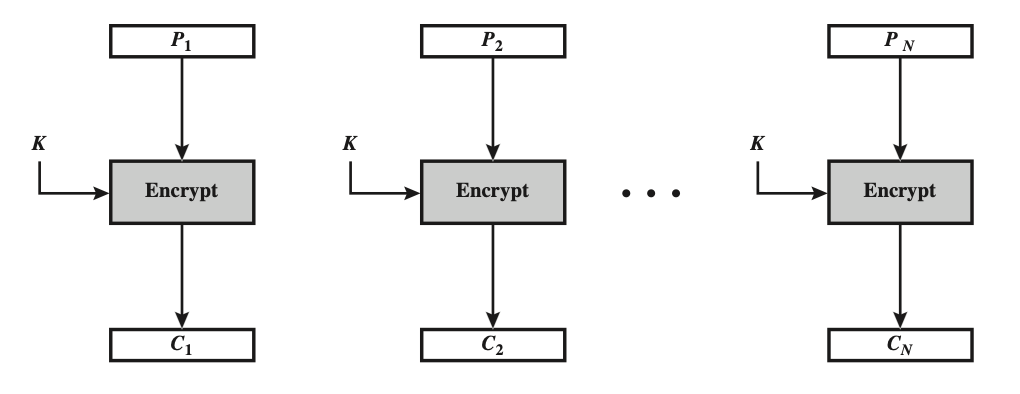
\includegraphics[width=0.5\textwidth]{img/electriccodeblock.png}
    \caption{Electronic Code Book}
\end{figure}

\subsection{Cipher Block Chaining}

La modalità di funzionamento ``Cipher Block Chaining'' (\verb|CBC|) è un metodo
di crittografia a blocchi che introduce un certo grado di indipendenza tra i
blocchi di testo in chiaro durante il processo di crittografia. Funziona come
segue:

\begin{enumerate}
    \item Prima di crittografare, viene generato un vettore di inizializzazione
    casuale noto come vettore di inizializzazione (\texttt{IV}). Questo vettore
    è combinato con il primo blocco di testo in chiaro tramite un'operazione di
    \texttt{XOR}.
    
    \item Il risultato di questa operazione \texttt{XOR} viene quindi
    crittografato utilizzando l'algoritmo di cifratura a blocchi insieme
    alla chiave.
    
    \item Il blocco di testo cifrato risultante viene poi combinato con il
    blocco di testo successivo prima della crittografia. Questo collegamento
    tra i blocchi di testo in chiaro aiuta a rompere la correlazione tra i
    blocchi di testo in chiaro, migliorando la sicurezza rispetto alla modalità
    di Electronic Code Book (\texttt{ECB}).
    
    \item Questo processo continua per tutti i blocchi di testo in chiaro
    successivi, garantendo che ciascun blocco di testo cifrato dipenda dal
    blocco di testo in chiaro precedente, oltre che dalla chiave.
\end{enumerate}

La decodifica avviene seguendo lo stesso processo in ordine inverso,
utilizzando il vettore di inizializzazione e la chiave per ottenere il
testo in chiaro originale.

La modalità \texttt{CBC} è considerata più sicura dell'\texttt{ECB} poiché
introduce una
dipendenza tra i blocchi di testo in chiaro, rendendo più complessa l'analisi
statistica e aumentando la resistenza agli attacchi crittoanalitici.
Tuttavia, è importante gestire correttamente il vettore di inizializzazione
per garantire la sicurezza e l'integrità del sistema di crittografia.
\[ C_j = E(K, [C_{j-1} \oplus P_j]) \]
\begin{figure}[H]
    \centering
    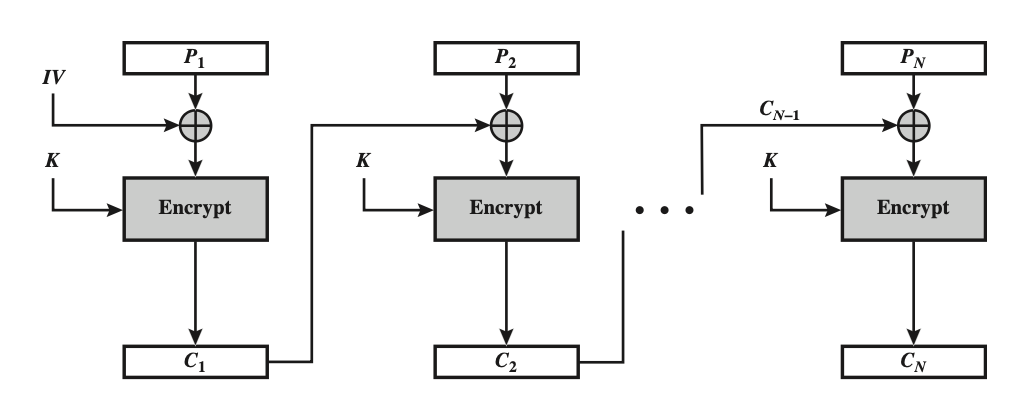
\includegraphics[width=0.8\textwidth]{img/CBC.png}
    \caption{Cipher Block Chaining}
\end{figure}
\subsection{Cipher Feedback}
Per \verb|AES|, \verb|DES| o qualsiasi altro cifrario a blocchi, la crittografia viene eseguita
su un blocco di \(b\) bit. Nel caso di \verb|DES|, \(b = 64\), e nel caso di \verb|AES|,
\(b = 128\). Tuttavia, è possibile convertire un cifrario a blocchi in un cifrario
a flusso utilizzando una delle modalità di funzionamento: la modalità di
Feedback di Cifratura (\verb|CFB|) e la modalità di Feedback di Output (\verb|OFB|).

Un cifrario a flusso elimina la necessità di aggiungere padding a un messaggio
per renderlo un numero intero di blocchi. Inoltre, può funzionare in tempo reale.
Pertanto, se viene trasmesso uno stream di caratteri, ogni carattere può essere
cifrato e trasmesso immediatamente utilizzando un cifrario a flusso orientato
ai caratteri.

Una proprietà desiderabile di un cifrario a flusso è che il testo cifrato abbia
la stessa lunghezza del testo in chiaro. Pertanto, se vengono trasmessi caratteri
di $8$ bit, ogni carattere dovrebbe essere cifrato per produrre un output di
testo cifrato di $8$ bit. Se vengono prodotti più di $8$ bit, la capacità di
trasmissione viene sprecata.

La modalità \verb|CFB| è illustrata nello schema. In questa modalità, il testo in chiaro
è diviso in segmenti di \(s\) bit, dove \(s\) è la dimensione dell'unità di
trasmissione. Durante la crittografia, viene utilizzato un registro a scorrimento
di \(b\) bit inizializzato con un vettore di inizializzazione (\verb|IV|). I
primi \(s\) bit più significativi dell'output della funzione di crittografia
vengono combinati con il primo segmento di testo in chiaro \(P_1\) tramite
l'operazione \texttt{XOR} per produrre l'unità di testo cifrato \(C_1\), che viene quindi
trasmessa. Il contenuto del registro a scorrimento viene spostato a sinistra di
\(s\) bit e \(C_1\) viene inserito nei \(s\) bit meno significativi del registro
a scorrimento. Questo processo continua fino a quando tutti i segmenti di testo
in chiaro sono stati crittografati.

Per la decodifica, viene utilizzato lo stesso schema, ad eccezione che l'unità
di testo cifrato ricevuta viene combinata tramite \verb|XOR| con l'output della funzione
di crittografia per produrre l'unità di testo in chiaro. È importante notare che
viene utilizzata la funzione di crittografia e non quella di decodifica. Questo
è facilmente spiegabile. Sia \(\texttt{MSBs}(X)\) definita come i \(s\) bit più significativi
di \(X\). Quindi

\[ C_1 = P_1 \oplus \texttt{MSBs}[E(K, IV)] \]

Di conseguenza, riarrangiando i termini:

\[ P_1 = C_1 \oplus \texttt{MSBs}[E(K, IV)] \]
\begin{figure}[H]
    \centering
    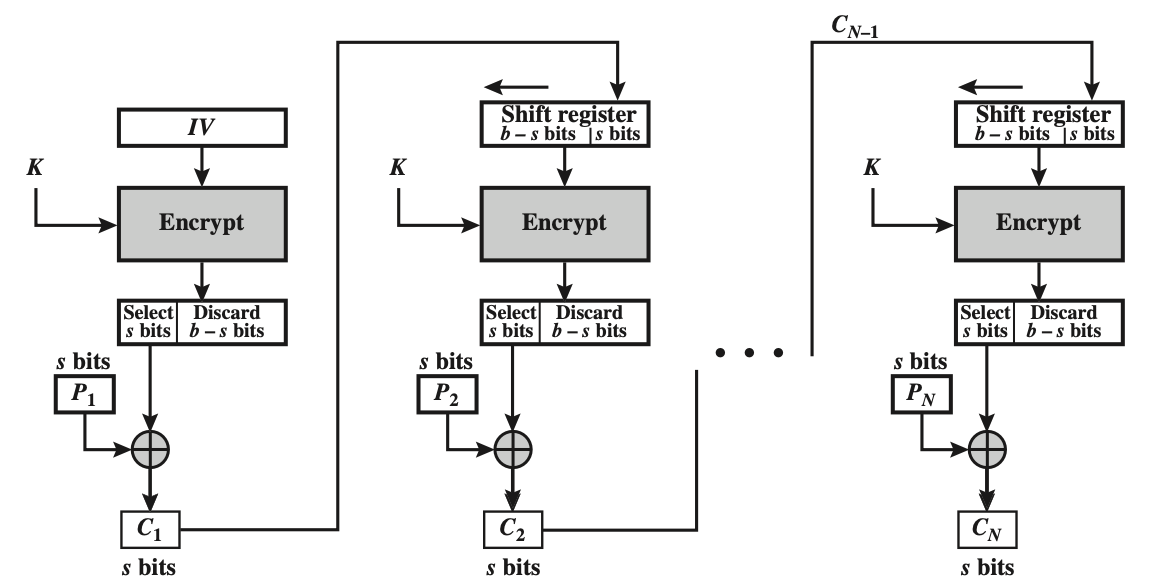
\includegraphics[width=0.8\textwidth]{img/cipherFeedback.png}
    \caption{Cipher Feedback}
\end{figure}
\subsection{Output Feedback}
La modalità di Feedback di Output (\verb|OFB|) ha una struttura simile a
quella di \verb|CFB|. Per \verb|OFB|, l'output della funzione di crittografia viene
retroalimentato e diventa l'input per crittografare il blocco successivo
di testo in chiaro. In \verb|CFB|, l'output dell'unità \verb|XOR| viene
retroalimentato e diventa l'input per crittografare il blocco successivo.
L'altra differenza è che la modalità \verb|OFB| opera su blocchi completi
di testo
in chiaro e testo cifrato, mentre \verb|CFB| opera su un sottoinsieme di \(s\) bit.
La crittografia \verb|OFB| può essere espressa come:

\[ C_j = P_j \oplus E(K, O_{j-1}) \]
\[ O_{j-1} = E(K, O_{j-2}) \]

Un po' di riflessione dovrebbe convincerti che possiamo riscrivere
l'espressione di crittografia come:

\[ C_j = P_j \oplus E(K, [C_{j-1} \oplus P_{j-1}]) \]

Riarrangiando i termini, possiamo dimostrare che la decodifica funziona:

\[ P_j = C_j \oplus E(K, [C_{j-1} \oplus P_{j-1}]) \]

\begin{figure}[H]
    \centering
    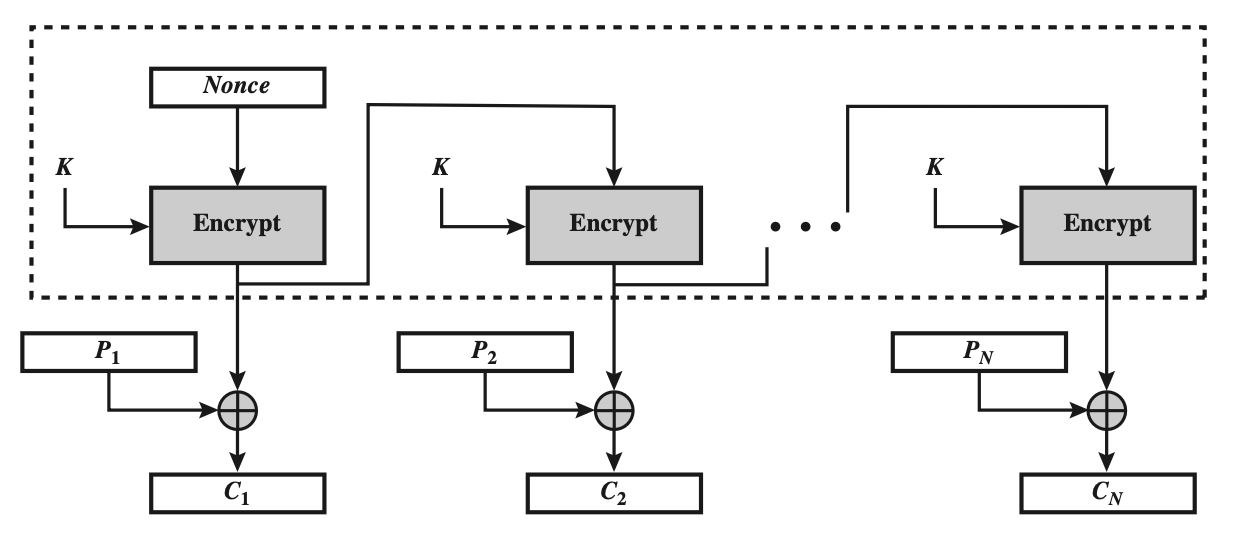
\includegraphics[width=0.8\textwidth]{img/outputFeedback.png}
    \caption{Output Feedback}
    \label{fig:outputFeedback}
\end{figure}
I blocchi di output della cifratura, \(O_i\), dipendono solo dalla chiave
e dal vettore di inizializzazione (\verb|IV|) e non dipendono dal testo
in chiaro. Pertanto, per una data chiave e \verb|IV|, lo stream di bit di
output utilizzato per l'operazione \texttt{XOR} con lo stream di bit in chiaro è fisso.
Se due messaggi diversi avessero un blocco identico di testo in chiaro
nella stessa posizione, un attaccante sarebbe in grado di determinare
quella parte dello stream \(O_i\).

Un vantaggio del metodo \verb|OFB| è che gli errori di bit nella trasmissione non
si propagano. Ad esempio, se si verifica un errore di bit in \(C_1\), solo
il valore ripristinato di \(P_1\) viene influenzato; i blocchi di testo in
chiaro successivi non vengono corrotti. Con \verb|CFB|, \(C_1\) serve anche come
input al registro a scorrimento e quindi causa corruzioni aggiuntive a valle.

Lo svantaggio di \verb|OFB| è che è più vulnerabile a un attacco di modifica dello
stream di messaggi rispetto a \verb|CFB|. Considera che complementare un bit nel
testo cifrato complementa il bit corrispondente nel testo in chiaro
ripristinato. Pertanto, possono essere effettuate modifiche controllate
al testo in chiaro ripristinato. Questo potrebbe rendere possibile per un
avversario, apportando le modifiche necessarie alla parte di checksum del
messaggio e alla parte di dati, modificare il testo cifrato in modo che non
sia rilevato da un codice di correzione degli errori.

\verb|OFB| ha la struttura di un tipico cifrario a flusso, poiché il cifrario
genera uno stream di bit come funzione di un valore iniziale e di una chiave,
e questo stream di bit viene operato con \verb|XOR| con i bit del testo in chiaro.
Lo stream generato che viene operato con \verb|XOR| con il testo in chiaro è
indipendente dal testo in chiaro stesso; questo è evidenziato da riquadri
tratteggiati in Figura (\ref{fig:outputFeedback}). Una differenza rispetto
ai cifrari a flusso è che \verb|OFB| crittografa il testo in chiaro un blocco
intero alla volta, dove tipicamente un blocco è di $64$ o $128$ bit. Molti
cifrari a flusso crittografano un byte alla volta.

\section{Rete di Feistel}
Moltissimi algoritmo di cifratura a blocchi utilizzano tale struttura.
La struttura di Feistel è una struttura di rete iterativa che è stata
progettata per essere utilizzata in cifrari a blocchi.
Tale struttura ha delle caratteristiche distintive:
\begin{itemize}
    \item L'input viene diviso in due metà.
    \item Esegue molteplici \textit{round} di cifratura, dove in ogni round 
    le due metà vengono elaborate in modo come segue:
    \begin{itemize}
        \item La metà sinistra diventa la metà destra del round precedente.
        \[
          L_i = R_{i-1}  
        \]
        \item La metà destra diventa l'applicazione della funzione di \texttt{XOR}
        tra la metà sinistra del round precedente e l'output della funzione $f$ che prende 
        in input la metà destra del round precedente e la chiave del round precedente.
        \[
            R_i = L_{i-1} \oplus f(R_{i-1}, K_{i-1})
        \]
    \end{itemize}
    \item La struttura è simmetrica, il che significa che la decodifica 
    avviene semplicemente invertendo l'ordine delle chiavi usate per la cifratura.
    \begin{itemize}
        \item \[ R_{i-1} = L_i \]
        \item \[L_{i-1} = R_i \oplus f(L_i, K_i)\]
    \end{itemize}
\end{itemize}
Il vantaggio è che le funzioni $f$ usate sono \textbf{one-way}.
\begin{tcolorbox}[title=One-way function]
    Una funzione $f: \{0,1\}^* \rightarrow \{0,1\}^*$ è \textbf{one-way} se esiste un algoritmo 
    che in tempo polinomiale mappa $x$ in $f(x)$ per ogni $x \in \{0,1\}^*$ e per ogni algoritmo 
    probabilistico polinomiale $\mathcal{A}$, ogni polinomio $p(\cdot)$
    e ogni intero $n$ sufficientemente grande, si ha che la probabilità che $\mathcal{A}$
    trovi un $x$ tale che $f(\mathcal{A}(f(x))) = f(x)$ è minore di $1/p(n)$.
\end{tcolorbox}
Anche se un algoritmo ha accesso a un metodo efficiente per generare valori che, una volta
processati dalla funzione $f$, producono un output, è estremamente improbabile che tale algoritmo 
possa invertire la funzione e trovare l'input originale dato l'output, almeno senza una 
quantità impraticabile di tempo e risorse.
\begin{figure}[H]
    \centering
    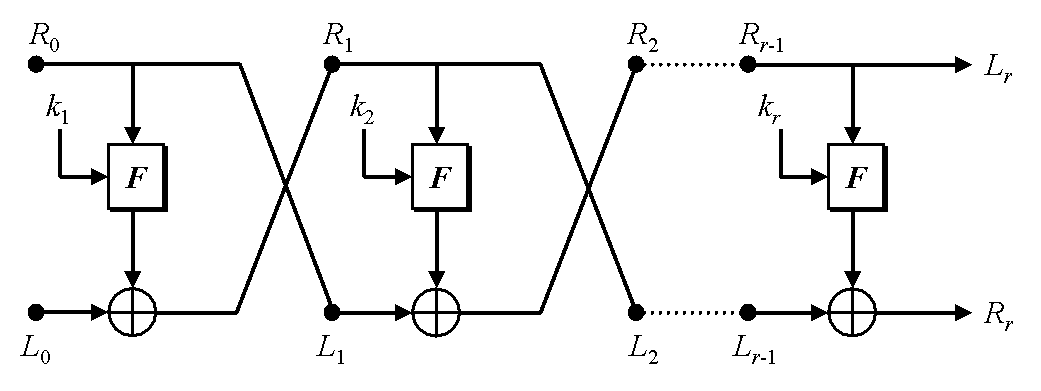
\includegraphics[width=0.8\textwidth]{img/feistel.png}
    \caption{Rete di Feistel}
\end{figure}
\section{Data Encryption Standard - \texttt{DES}}
\texttt{DES} è un cifrario a blocchi a chiave simmetrica che utilizza una struttura di Feistel.

La chiave è di $56$ bit, ma in realtà sono $64$ bit, di cui $8$ sono di parità, ed 
opera su blocchi di $64$ bit. 
L'algoritmo esegue una permutazione iniziale dei bit del blocco di testo in chiaro,
nota come \textit{Initial Permutation (IP)}, che riordina i bit secondo uno schema
fisso predefinito. Questo è seguito da 16 round di cifratura che consistono in espansione,
mescolamento con una chiave di round derivata dalla chiave principale, sostituzione tramite S-Box
e una permutazione finale. La funzione di round prende input dalla metà destra del blocco di dati
e la chiave di round, producendo un output che è poi combinato con la metà sinistra attraverso
un'operazione XOR.

Dopo l'ultimo round, le due metà del blocco vengono scambiate, e questo è seguito da una
\textit{Final Permutation (FP)}, che è l'inverso della permutazione iniziale. Il risultato
è il blocco di testo cifrato. La decodifica con \texttt{DES} segue lo stesso processo ma
in ordine inverso, utilizzando le chiavi di round in ordine inverso.

Nonostante la sua ampiamente testata sicurezza, la principale vulnerabilità di \texttt{DES}
risiede nella lunghezza della chiave. Tecniche come l'attacco a forza bruta, che era
teoricamente possibile ma non praticabile al tempo della sua creazione, sono divenute
fattibili con l'avanzamento della potenza di calcolo. Per questo motivo, \texttt{DES}
è stato sostituito da \texttt{AES} come standard approvato dal NIST (\textit{National
Institute of Standards and Technology}) per la cifratura di informazioni sensibili.
\subsection{Funzione di round}
La funzione di round prende in input $32$ bit e una chiave di round di $48$ bit e produce
un output di $32$ bit. La funzione di round è composta da quattro passaggi:
\begin{enumerate}
    \item \textbf{Espansione}: i $32$ bit di input vengono espansi a $48$ bit tramite una
    permutazione fissa.
    \item \textbf{Mescolamento}: i $48$ bit vengono combinati con la chiave di round tramite
    un'operazione di \texttt{XOR}.
    \item \textbf{Sostituzione}: Dopo il mescolamento con la chiave di round, i $48$ bit vengono
    passano attraverso $8$ \texttt{S-BOX}, ciascuno dei quali sostituisce $6$ bit con $4$ bit. 
    Sono lineari e complesse per aggiungere sicurezza alla cifratura.
    \item \textbf{Permutazione}: i $32$ bit vengono permutati tramite una permutazione fissa.
\end{enumerate}
L'alternanza di sostituzioni mediante \texttt{S-BOX}, permutazioni mediante permutazioni fisse
e espansioni forniscono la \textbf{confusione} e la \textbf{diffusione}, concetti introdotti
da \texttt{Shannon} e che sono alla base di molti cifrari moderni.

\begin{tcolorbox}[title=Confusione]
    Si tratta della relazione tra il testo in chiaro e la chiave. Deve essere difficile
    dedurre la chiave a partire dal testo cifrato. Ogni bit del testo cifrato deve
    dipendere da molti bit della chiave.
\end{tcolorbox}

\begin{tcolorbox}[title=Diffusione]
    Si tratta della capacità di un algoritmo di distribuire le correlazioni statistiche
    del testo lungo tutto l'alfabeto utilizzato dall'algoritmo di cifratura, rendendo quanto 
    più difficile un attacco statistico.
\end{tcolorbox}
\end{document}
